\documentclass[12pt]{article}

\usepackage{graphicx}
\usepackage{pdfpages}
\usepackage{listings}
\usepackage{amsmath}
\usepackage{amsfonts}
\usepackage{subcaption}

\renewcommand{\figurename}{Fig.}
\renewcommand{\contentsname}{Innhold}

\title{TTK4260 Innføring i Multivariat Datamodellering}
\date{}
\author{Kristian Løvland}

\begin{document}

\maketitle
\tableofcontents

\newpage
\section{Introduksjon}
Dette dokumentet er et forsøk på å skaffe meg en strukturert oversikt over et middels strukturert fag. Ting er først og fremst hentet fra slides, men også noe fra lærebøker jeg kanskje legger til som kilder senere.

\newpage
\section{Grunnleggende statistikk}
Til grunn for alle multivariate metoder som kommer senere, ligger den grunnleggende statistikken som forhåpentligvis er kjent fra før. Den oppsummeres her i korte trekk.

\subsection{Kort om notasjon}
Gjennom denne oppsummeringen brukes følgende notasjon
\begin{itemize}
\item Skalare variabler og funksjoner skrives med små bokstaver -- $\alpha, x, g(\cdot)$
\item Vektorvariabler og -funksjoner skrives med små, fete bokstaver -- $\mathbf{\alpha}, \mathbf{x}, \mathbf{g(\cdot)}$
\item Matriser skrives med store bokstaver -- $A, X$
\item Transponert, invers, pseudoinvers -- $\cdot^T, \cdot^{-1}, \cdot^\dagger$
\item Definisjonsmengder skrives med kaligrafiske bokstaver, eller stor theta -- $\mathcal{X}, \mathcal{Y}, \mathcal{D}$ eller $\Theta$
\end{itemize}

\subsection{Definisjoner}
En funksjon \(\phi(\boldsymbol{y}): \mathcal{Y}^{N} \mapsto \mathbb{R}^{M}\) er en \textbf{observator} dersom den er målbar, og den er uavhengig av $\theta$. En observator \(\phi(\boldsymbol{y}): \boldsymbol{y}^{N} \mapsto \Theta\) er en \textbf{estimator} dersom den er målbar og uavhengig av $\theta$ (dvs. den er en observator med verdimengde lik $\Theta$.

\subsection{Antagelser}
Når vi snakker om regresjon, antar vi at dataen $y_t$ genereres av funksjonen \(y_{t}=f\left(u_{t} ; \theta\right)+v_{t}\), og at dette resulterer i et datasett \(\mathcal{D}=\left\{\left(u_{t}, y_{t}\right)\right\}_{t=1, \ldots, N}\). Ved hjelp av parametre \(\theta \in \Theta\), hypoteserommet vårt, vil vi finne en estimator \(\widehat{\theta} \in \Theta\) som best mulig forklarer datasettet vårt.

Hva betyr det å "best mulig forklare $\mathcal{D}$? Det finnes det ulike tolkninger av.

\subsection{Minste kvadrater}
En naturlig tolkning av spørsmålet om å best mulig forklare datasettet vha $\theta$, er å finne parameteren som ved bruk av vår antatte modell $f(u_t; \theta)$, gir den korteste avstanden fra predikert datasett til faktisk datasett. "Avstand" har her den vanlige, euklidiske tolkningen, slik at en minste kvadraters estimator av en parameter $\theta$ gitt et datasett $\mathcal{D}$ og en modell $f(u_t; \theta)$, er gitt av
\begin{equation}
\widehat{\theta}_{\mathrm{LS}}=\arg \min _{\theta \in \Theta}\left\|\left[\begin{array}{c}
{y_{1}} \\
{\vdots} \\
{y_{N}}
\end{array}\right]-\left[\begin{array}{c}
{f\left(u_{1} ; \theta\right)} \\
{\vdots} \\
{f\left(u_{N} ; \theta\right)}
\end{array}\right]\right\|^{2}=\arg \min _{\theta \in \Theta} \sum_{t=1}^{N}\left(y_{t}-f\left(u_{t} ; \theta\right)\right)^{2}
\end{equation}
En nyttig verdi som følger av dette estimatet er residualen $r_{t}(\theta):=y_{t}-f\left(u_{t} ; \theta\right)$.

En nyttig klasse av problemer er de \textbf{separable} problemene. Disse er på formen
\begin{equation}
y_{t}=\sum_{j=1}^{n} \theta_{j} \phi_{j}\left(u_{t}\right)+e_{t}
\end{equation}
Dvs. at parameterne som skal estimeres inngår lineært i modellen vår. Da kan $\phi(u_t)$ være så komplisert den vil, LS-problemet vil uansett reduseres til et lineært likningssett på formen
\begin{equation}
\left[\begin{array}{c}
{y_{1}} \\
{\vdots} \\
{y_{N}}
\end{array}\right]=\left[\begin{array}{ccc}
{\phi_{1}\left(u_{1}\right)} & {\cdots} & {\phi_{n}\left(u_{1}\right)} \\
{\vdots} & {} & {\vdots} \\
{\phi_{1}\left(u_{N}\right)} & {\cdots} & {\phi_{n}\left(u_{N}\right)}
\end{array}\right]\left[\begin{array}{c}
{\theta_{1}} \\
{\vdots} \\
{\theta_{n}}
\end{array}\right]+\left[\begin{array}{c}
{e_{1}} \\
{\vdots} \\
{e_{N}}
\end{array}\right]
\end{equation}
Som mer kompakt kan skrives som
\begin{equation}
\boldsymbol{y}=\Phi(\boldsymbol{u}) \boldsymbol{\theta}+\boldsymbol{e}
\end{equation}
Målet vårt er å minimere $\mathbf{e}$. Dette kan gjøres vha. lineær programmering, men om vi ikke har begrensninger i $\theta$, dvs. $\Theta = \mathbb{R}^n$ for en eller annen $n$, kan dette løses eksplisitt som
\begin{equation}
\widehat{\theta}_{\mathrm{LS}}=\arg \min _{\boldsymbol{\theta} \in \mathbb{R}^{n}}\|\boldsymbol{y}-\Phi(\boldsymbol{u}) \boldsymbol{\theta}\|^{2}
\end{equation}
Ved å derivere dette og sette det lik null får vi \textbf{normallikningene}
\begin{equation}
\Phi(\boldsymbol{u})^{T} \Phi(\boldsymbol{u}) \widehat{\theta}_{\mathrm{LS}}=\Phi(\boldsymbol{u})^{T} \boldsymbol{y}
\end{equation}
Men hva om $
\Phi(\boldsymbol{u})^{T} \Phi(\boldsymbol{u})
$ ikke er invertibel? Da vil ikke normallikningene ha noen entydig løsning. Dette ordner vi ved å bruke \textbf{pseudoinversen}, som har noen kjekke egenskaper (nærmeste løsning hvis ingen løsning eksisterer, løsning med minst norm hvis mange løsninger eksisterer).

Noen ganger er imidlertid ikke alle tilstander like viktige. Dette løser vi ved å multiplisere hver feil med en vekt, slik at minimeringsproblemet (for ubegrensede problemer) blir
\begin{equation}
\widehat{\theta}_{\mathrm{WLS}}=\arg \min _{\boldsymbol{\theta} \in \mathbb{R}^{n}}(\boldsymbol{y}-\Phi(\boldsymbol{u}) \boldsymbol{\theta})^{T} W(\boldsymbol{y}-\Phi(\boldsymbol{u}) \boldsymbol{\theta})
\end{equation}
Mer kompakt kan dette skrives som $
=\arg \min _{\boldsymbol{\theta} \in \mathbb{R}^{n}}\|\boldsymbol{y}-\Phi(\boldsymbol{u}) \boldsymbol{\theta}\|_{W^{-1}}^{2}
$. Et nytt sett med normalligninger faller ut av dette, nå blir 
\begin{equation}
\Phi(\boldsymbol{u})^{T} W \Phi(\boldsymbol{u}) \boldsymbol{\theta}=\Phi(\boldsymbol{u})^{T} W \boldsymbol{y}
\end{equation}
som kan løses likt som tidligere, f.eks. med pseudoinvers.

Hva om problemet vårt er ulineært (ikke separabelt)? Optimeringsproblemet kan fortsatt være veldefinert, og da kan det løses numerisk. MATLAB gjør dette med \texttt{fmincon}, og de fleste programmeringsspråk med respekt for seg selv har rammeverk som gjør det samme.

\subsection{Maksimal sannsynlighet}
Forrige avsnitt ga en rent geometrisk tolkning av minste kvadrater. Ofte har min imidlertid kunnskap om de statistiske egenskapene til støyen og feilen som forsøpler dataen din, og denne informasjonen er gjerne nyttig å bruke. Utgangspunktet for dette er sannsynlighetsfordelingen, skrevet som $p(y ; \theta)$. Ofte operer man med $\theta$ fiksert og $y$ varierende. I vårt tilfelle er $y$ gitt (den utgjør datasettet vårt $\mathcal{D}$, og vi er ute etter å finne en $\theta$ som best forklarer dette. Da kalles $p(y ; \theta)$ for \textbf{sannsynlighet}.

Med dette definert er vi klare for å definere vår maksimale sannsynlighetsestimator
\begin{equation}
\widehat{\theta}_{\mathrm{ML}}=\arg \max _{\theta \in \Theta} p(\mathcal{D} ; \theta)
\end{equation}
Vi ser at denne ligner i formen på LS-estimatoren, men at funksjonen $p$ gir oss mer valgfrihet, og muligheter til å inkludere kjent informasjon om modell og data.

Det er verdt å merke seg at et ML-estimat ikke nødvendigvis trenger å eksistere. Man kan komme opp med massevis av eksempler på at denne ikke eksiterer, f.eks. kan man la $\Theta$ er en åpen mengde. Hvis $p$ er kontinuerlig og $\Theta$ er kompakt tror jeg imidlertid vi kan føle oss ganske trygge, i hvert fall hvis man er av typen som stoler på det Weierstrass hadde å si oss.

Et viktig eksempel på en ML-estimator er når $p$ er normalfordelt. Da vil sannsynlighetsfunksjonen til et datasett være gitt av
\begin{equation}
p\left(y_{1}, \ldots, y_{N} ; m, \sigma^{2}\right)=\prod_{t=1}^{N} p\left(y_{t} ; m, \sigma^{2}\right)=\prod_{t=1}^{N}\left(\frac{1}{\sqrt{2 \pi \sigma^{2}}} \exp \left(-\frac{1}{2} \frac{\left(y_{t}-m\right)^{2}}{\sigma^{2}}\right)\right)
\end{equation}
Dette grumsete uttrykket motiverer definisjonen av log-sannsynlighetsfunksjonen. Siden $\log(\cdot)$-funksjonen er monotont stigende i input-argumentet sitt, vil maksimerende input til funksjonen være lik maksimerende input til logaritmen av funksjonen. Vi definerer
\begin{equation}
\ell(\theta):=-\log p(\mathcal{D} ; \theta)
\end{equation}
I eksempelet med normalfordelt $p$ vil vi nå kunne formulere
\begin{equation}
\widehat{\theta}_{\mathrm{ML}}=\arg \max _{\theta \in \Theta} p(\mathcal{D} ; \theta) = \arg \min _{\theta \in \Theta} \ell(\theta)
\end{equation}
Eksponential- og logaritmefunksjonen spiller hverandre gode, og ved litt regning kan man se at
\begin{equation}
\arg \min _{m \in \mathbb{R}, \sigma^{2} \in \mathbb{R}_{+}} \ell\left(m, \sigma^{2}\right)=\arg \min _{m \in \mathbb{R}, \sigma^{2} \in \mathbb{R}_{+}} N \log \left(\sigma^{2}\right)+\frac{\sum_{t=1}^{N}\left(y_{t}-m\right)^{2}}{\sigma^{2}}
\end{equation}
Dennes gradient settes lik null, men her vil det inngå informasjon vi ikke har tilgang på. Vi ender opp med å benytte estimatene, og får
\begin{equation}
\bar{m}=\frac{1}{N} \sum_{t=1}^{N} y_{t}
\end{equation}
\begin{equation}
\bar{\sigma}^{2}=\frac{1}{N} \sum_{t=1}^{N}\left(y_{t}-\bar{m}\right)^{2}
\end{equation}
som ser fornuftig ut.

\subsection{Maksimal a posteriori}
Vi begynner med Bayes' lov
\begin{equation}
P(A | B)=\frac{P(A B)}{P(B)} = \frac{P(B | A) P(A)}{P(B)}
\end{equation}
som kan bevises ved Venn-diagram eller lignende.

Ved å bytte ut $A$ og $B$ med $\theta$ og $y$, får vi en måte å oppdatere vår tro om en variabel sin fordeling på, basert på data. Vi er imidlertid avhengige av å ha en initiell formening om fordelingen til $\theta$, dette kalles en \textbf{prior}. I praksis vil denne gjerne gjøre få antagelser, men utelukke fullstendig urealistiske muligheter (f.eks. utelukke negativ høyde på personer, om man vil estimere dette). Med en modell $P(y | \theta)$, en prior $P(\theta)$, og data som gir oss $P(y)$, får vi da
\begin{equation}
P(\theta | y)=\frac{P(y | \theta) P(\theta)}{P(y)}
\end{equation}
Basert på denne nye, evidensbaserte fordelingen, kan vi definere estimatoren
\begin{equation}
\widehat{\theta}_{\mathrm{MAP}}:=\arg \max _{\theta \in \Theta} P(\theta | y)=\arg \max _{\theta \in \Theta} \frac{P(y | \theta) P(\theta)}{P(y)}=\arg \max _{\theta \in \Theta} P(y | \theta) P(\theta)
\end{equation}
som vil være moden til den posteriore fordeling. Merk at denne ikke trenger å være representativ for fordelingen, f.eks. hvis fordelingen har en smal, høy topp langt unna "tyngdepunktet".

\subsection{Statistiske ytelsesindekser}
Det nevnes tre bruksområder for indekser som måler statistisk ytelse
\begin{itemize}
\item Regresjonsproblemer
\item Klassifiseringsproblemer
\item Sammenligning av sannsynlighetsfordelinger
\end{itemize}
Vi går gjennom disse i den rekkefølgen.

\subsubsection{Regresjonsproblemer}
En naturlig indeks er \textbf{Mean Squared Error (MSE)}
\begin{equation}
\textrm{MSE} = \mathbb{E}\left[\|\theta-\widehat{\theta}\|^{2}\right]
\end{equation}

Av denne følger \textbf{Root Mean Square Error}
\begin{equation}
\textrm{RMSE} = \sqrt{\mathbb{E}\left[\|\theta-\widehat{\theta}\|^{2}\right]}
\end{equation}

Det er viktig å merke seg at siden MSE er en funksjon av $\theta$, så kan den ikke regnes ut. Hvorfor bryr vi oss om den da? Tja, den kan i hvert fall inspirere lignende indekser. \textbf{Residual Sum of Squares (RSS)} baserer seg på residualene til estimatene
\begin{equation}
\operatorname{RSS}(\widehat{\theta}):=\sum_{i}\left(y_{i}-\widehat{y}_{i}(\widehat{\theta})\right)^{2}
\end{equation}

Det finnes imidlertid problemer med alle disse. Først og fremst er det et problem at de er avhengig av mengden av og størrelsen på dataen man vurderer estimatene av. Man vektlegger å unngå avvik i estimatene fra store målinger mer enn små. En metode som fungerer noe bedre, uten å bruke normalisering, er å bruke 1-normen i stedet for kvadratet. Dette gjøres i \textbf{Mean Absolute Deviaton (MAD)}
\begin{equation}
\mathrm{MAD}:=\mathbb{E}[|y-\widehat{y}|]
\end{equation}

En metode som bruker en form for normalisering er \textbf{Fraction of Variance Unexplained (FVU)}
\begin{equation}
\mathrm{FVU}(\widehat{\theta}):=\frac{\operatorname{RSS}(\widehat{\theta})}{\operatorname{var}(y)}=\frac{\sum_{i}\left(y_{i}-\widehat{y}_{i}(\widehat{\theta})\right)^{2}}{\sum_{i}\left(y_{i}-\frac{1}{N} \sum_{i} y_{i}\right)^{2}}
\end{equation}
Denne må tolkes med måte, siden hva som er en god forklaringgrad er veldig avhengig av hva slags felt man jobber i, og det konkrete bruksområdet. Dette er uansett en mye brukt indeks, men da i form av $R^{2}$
Denne tolkes som "andel av variansen i avhengig variable som er predikerbar fra de uavhengige variablene".

\subsubsection{Klassifiseringsproblemer}
Vi diskuterer her klassifisering i form av "ja/nei". Da kan man gjøre to typer feil: Falsk positiv (\textbf{Type 1}) og falsk negativ (\textbf{Type 2}). Figur \ref{fig:klassifisering} viser definisjonen på en del uttrykk som beskriver egenskapene til en klassifikator.

\begin{figure}[h]
\centering
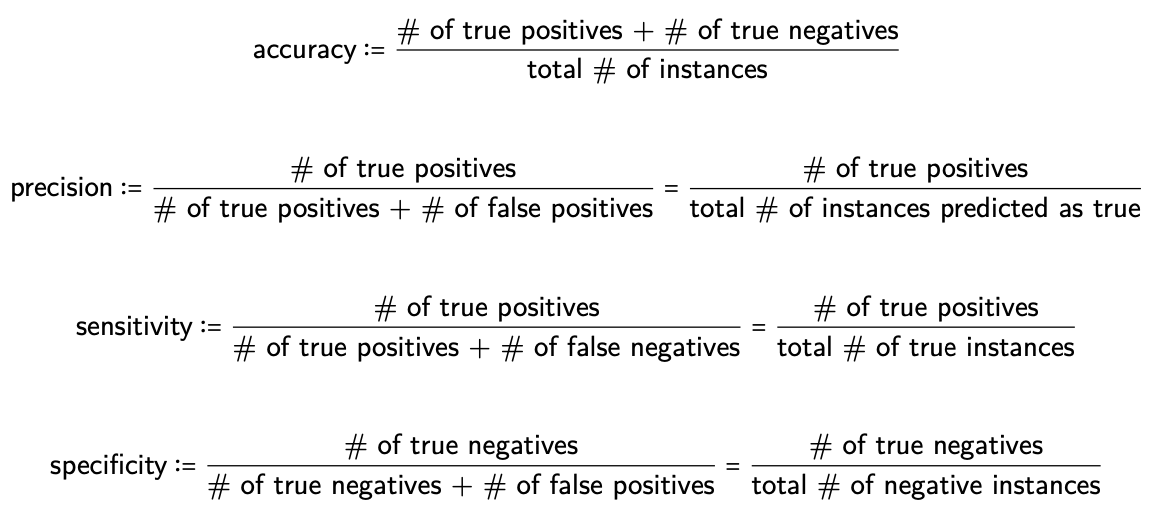
\includegraphics[width=0.8\textwidth]{klassifisering.png}
\caption{Egenskaper til klassifikator}
\label{fig:klassifisering}
\end{figure}

Muntlig kan disse forklares som
\begin{itemize}
\item \textbf{Prevalens} -- Hvor ofte opptrer ja-tilfellet i datasettet vårt?
\item \textbf{Nøyaktighet} -- Hvor ofte har klassifikatoren rett?
\item \textbf{Feilklassifiseringsrate} -- Hvor ofte tar klassifikatoren feil?
\item \textbf{Presisjon} -- Når klassifikatoren gjetter ja, hvor ofte er dette rett?
\item \textbf{Falsk positiv-rate} -- Når svaret er nei, hvor ofte gjetter klassifikatoren ja?
\item \textbf{Sensitivitet} -- Når svaret er ja, hvor ofte gjetter klassifikatoren ja?
\item \textbf{Spesifitet} -- Når svaret er nei, hvor ofter gjetter klassifikatoren nei?
\end{itemize}

Man kan også kombinere to av disse for å få \textbf{F1-score}
\begin{equation}
\textrm{F1-score} = 2 \frac{\textrm{presisjon} \cdot \textrm{
sensitivitet}}{\textrm{presisjon} + \textrm{
sensitivitet}}
\end{equation}

Om man vil finne ut hvor ulike to klassifikatorer er, kan man bruke \textbf{Kappa-koeffisient}. Dette forklares ikke mer, men det eksisterer.

\subsubsection{Sammenligning av sannsynlighetsfordelinger}
Her kan man bruke \textbf{Kullback-Leibler-divergens}.

\subsection{Bias vs. varians}
Dette er en avveining man ikke slipper unna når men bedriver estimering. La oss bruke MSE for å illustrere dette. La 

\begin{equation}
\begin{array}{l}{\mathcal{V}:=\widehat{\theta}-\mathbb{E}[\widehat{\theta}]} \\ {\mathcal{B}:=\mathbb{E}[\widehat{\theta}]-\theta}\end{array}
\end{equation}

\begin{align}
\mathbb{E}\left[\|\hat{\theta}-\theta\|^{2}\right] &=\mathbb{E}\left[\|\widehat{\theta}-\mathbb{E}[\widehat{\theta}]+\mathbb{E}[\widehat{\theta}]-\theta\|^{2}\right] \\ \nonumber
&=\mathbb{E}\left[\|\mathcal{V}+\mathcal{B}\|^{2}\right]\\ \nonumber
&=\mathbb{E}\left[(\mathcal{V}+\mathcal{B})^{T}(\mathcal{V}+\mathcal{B})\right] \\ \nonumber
&=\mathbb{E}\left[\|\mathcal{V}\|^{2}+\|\mathcal{B}\|^{2}+2 \mathcal{V}^{T} \mathcal{B}\right] \\ \nonumber
&=\mathbb{E}\left[\|\mathcal{V}\|^{2}\right]+\|\mathcal{B}\|^{2}
\end{align}

Denne avveiningen henger sammen med hvor komplisert man gjør forklaringsmodellen $f(u_t; \theta)$. Om man gjør den veldig komplisert vil man kunne følge dataen nøyaktig, men man vil være utsatt for at dette ikke lar seg generalisere til andre datasett \textbf{overfitting}. Dette svarer til lav bias, men stor varians. Om modellen er for enkel vil man få en enkel modell som generaliserer, men man vil også kunne unngå å beskrive viktig struktur i dataen. Dette er \textbf{underfitting}, og svarer til liten varians, men stor bias.

Det finnes flere metoder som forsøker å gjøre denne avveiningen. Noen av dem er
\begin{itemize}
\item Akaikes informasjonskriterium
\item Det Bayesiske informasjonskriteriumet
\item Minimum lengde-beskrivelse
\end{itemize}


\newpage
\section{Multivariat Dataanalyse}
Nå begynner vi på ekte her.

\subsection{Eksperimentdesign}


\end{document}